Many works on the area begin with the assertion that aspect is one of the most studied areas of linguistics \citep{Sasse2002RecentAI}, particularly Slavic linguistics (for reasons I will discuss later), and hence a thorough theoretical discussion of the linguistic phenomenon which does full justice to the work on the field is not possible within the constraints of this thesis. Nevertheless, in order to give an introduction to the fundamental elements of the following study and make a productive contribution to the area, I will touch on some of the main findings in the area of aspectology.
\section{A (short) phenomenology of aspect}
The Concise Oxford Dictionary of Linguistics \citep{matthews2014concise} defines aspect thus: 

\begin{quotation}
    [Aspect is a g]eneral term, originally of specialists in Slavic languages, for verbal categories that distinguish the status of events, etc. in relation to specific periods of time, as opposed to their simple location in the present, past, or future.
\end{quotation}

As noted here, one helpful distinction which must be made right away is that between \emph{aspect}, and another temporal phenomenon \emph{tense}. Many works recall Bernard Comrie's differentiation in his book \emph{Aspect} \citep{comrie1976aspect} between the deictic nature of \emph{tense} and the focus on the "internal temporal constituency of a situation" of \emph{aspect}. In other words: "tense\footnote{In many of the world's languages this is grammaticalised as past, present and future; in others such as English by some accounts \citep{jespersen2013essentials} it is a binary distinction such as past and non-past, whereas some languages such as Greenlandic (Kalaallisut) some linguists have even argued to be tenseless \citet{10.1093/jos/ffh029}. See also the contentious debate about Hopi time \citet{whorf-writings, hopitime}. } relates the time of the situation referred to to some other time, usually to the moment of speaking", and thus by relating the time of the situation to the time of the utterance it is deictic \citep{comrie1976aspect}. Aspect on the other hand gives a \emph{situation-internal} description of the events in that situation, such how they relate to each other temporally or how an individual event is temporally characterised. This introduces another important distinction: that between lexical and grammatical aspect.

\begin{figure}
    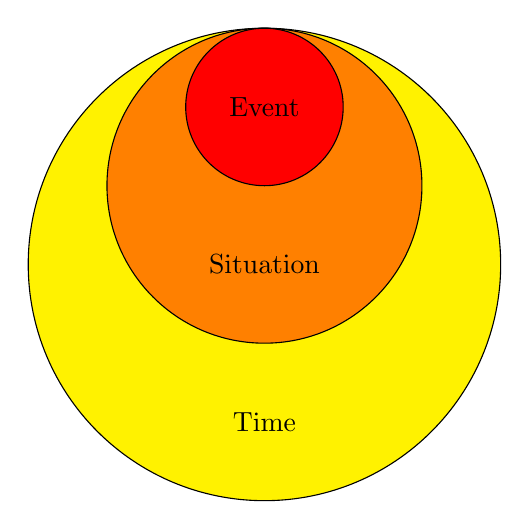
\begin{tikzpicture}
        \foreach \x/\z [count=\y] in {Time/yellow,Situation/orange,Event/red} {
            \draw[fill=\z] (0,{\y-4}) circle[radius={4-\y}];
            \node at (0,{-2*(4-\y)+1}) {\x};
        } 
    \end{tikzpicture}
    \hspace{2cm}
    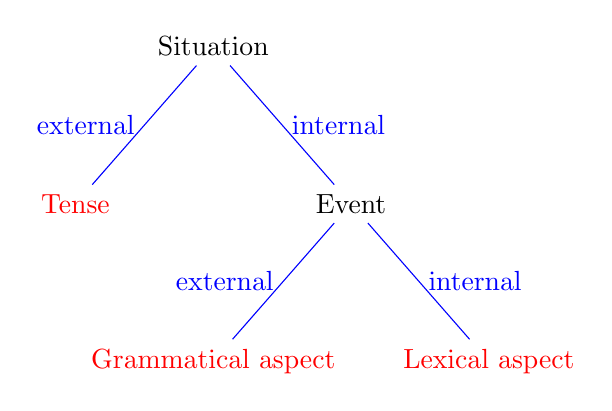
\begin{tikzpicture}
        \node {Situation}[sibling distance = 3.5cm, level distance = 2cm]
        child [red] {node {Tense} 
            edge from parent [blue] node [left] {external}}
        child {node {Event} 
            child [red] {node {Grammatical aspect}
                edge from parent [blue] node [left] {external}}
            child [red] {node {Lexical aspect}
                edge from parent [blue] node [right] {internal}} 
            edge from parent [blue] node [right] {internal}};
    \end{tikzpicture}
    \caption{A set-theoretical representation of the relationship between time, situation and event \emph{(left)} along with the categorisation of the three temporal phenomena discussed \emph{(right)}.}
    \label{fig:TimeSitEvent}
\end{figure}

\subsection{Lexical vs grammatical aspect}
The polysemy of the term “aspect” in the linguistic community is unfortunate. In an area of language which seems to have surprisingly far-reaching interactions with other parts of linguistic systems these ambiguities are particularly unhelpful.\footnote{Among other things, aspect is also intertwined with case, mood and voice \citep{franks2005slavic, Kiparsky2004PartitiveCA}.}
As already mentioned, aspect\footnote{Boogaart uses the term \emph{aspectuality} to remove the aforementioned ambiguity \citep{Boogaart+2004+1165+1180}. However, I will stick with the term \emph{aspect} due to its prevalence in the literature, further specifying where necessary.} is a term often used to refer to both lexical and grammatical aspect. Lexical aspect (also referred to as \emph{Aktionsart, situation aspect} or \emph{inner aspect}) is the inherent property of a verb or verb phrase which “characterizes the temporal profile of event descriptions” \citep{10.1093/oxfordhb/9780199601264.013.25}. For example, to “crack open an egg” is inherently a short event describing the change of one state (the egg being whole) to another (the egg being cracked). Grammatical aspect (or \emph{viewpoint aspect, outer aspect}), on the other hand, describes the “internal temporal constituency” \citep{comrie1976aspect} XCHANGE THIS!! of an event, such as its habituality or ongoing nature and can be seen more as an external lens imposed on a verbal phrase. In English, one example of this lens is the progressive, which is formed by the verb \emph{be} + gerund, as in the phrase “Sue was running”. 

Figure \ref{fig:TimeSitEvent} shows a taxonomy of tense, and grammatical and lexical aspect. An event is an atomic or 

Here each situation is a union of events ($\mathbf{situations} = \mathcal{P}(\mathbf{events}) \setminus \emptyset$) and the 

Situations are anchored in time. 

The concrete linguistic realisation of these categories is very often unclear or non-existent and exhibits a relatively wide variety of encodings throughout the world’s languages \citep{Dahl1985TenseAA}. It therefore proves tricky to uphold this distinction in empirical studies "in the real world". This has led some to question to what extent this distinction makes sense \citep{Sasse2002RecentAI}. Those who question the contrast between these two semantic dimensions, described as unidimensionalists in \citet{Sasse2002RecentAI}, claim that aspectual distinctions in both dimensions can be reduced to a common set of semantic primitives, which can be applied to all levels of analysis, i.e. the boundedness of lexical aspect is the same as the boundedness which marks the distinction between the perfective and imperfective parameters. 

I have chosen to introduce this distinction in order to WHAT

WHICH MODEL WOULD I LIKE TO USE IN THE END??

Nevertheless the theoretical differentiation of these two interrelated subdomains is an important one to make, and each describes a variety of concepts which will be useful later.

\subsection{Lexical aspect}
\subsection*{Telicity}
A fundamental distinction of lexical aspect is that of telicity (from Ancient Greek \emph{télos} meaning “end”). Telicity describes whether an event has an inherent goal or end-point after which the event can be regarded as completed: for example "go climbing" would be atelic whereas "climb the mountain" is telic (since it involves the agent reaching the summit of a mountain). A classic test for telicity\footnote{Though \citet{XiaoMcenery+2006+1+21} note that this test is flawed and propose an alternative test scheme.} is whether the verb phrase admits a completing adverb such as "in an hour" and does not admit a durative adverb such as "for an hour" \citep{Krifka1998TheOO}.

Dahl misleadingly defines telicity as "involv[ing] the presence of a boundary or the attainment of a specific result-state" \citep{DAHL2015210}, which, however can lead to confusion with the term \emph{(un)boundedness}.
\subsection*{Boundedness}
(Un)boundedness refers to the existance (or lack of) a \emph{temporal} boundary marking the end of an action. Boundedness must be distinguished from telicity\footnote{\citet{friedrich-etal-2023-kind} seem to mistakenly conflate the two, stating that "[t]elicity is also sometimes referred to as boundedness (e.g., by Loáiciga and Grisot, 2016)" referring to the 2016 paper \citet{loaiciga-grisot-2016-predicting}, which, however, clearly distinguishes between the two notions.} in order to avoid the so-called 'Imperfective Paradox' highlighted by \citet{Linguistics2005DowtyD1}, here verbalised by \citet{zucchi}:

\begin{quotation}
    How is it possible that a statement of the form \emph{x was F-ing} is true and yet there
    is no time at which \emph{x was F-ed} is true?
\end{quotation}
More concretely, it asks the question why (\ref{para1}) entails (\ref{para2}) but (\ref{para3}) doesn't entail (\ref{para4}) in the examples below:
\begin{exe}
    \ex The man was running.
    \label{para1}
    \ex The man ran.
    \label{para2}
    \ex The man was building a house.
    \label{para3}
    \ex The man built a house.
    \label{para4}
\end{exe}
\citet{6608d9d0-a477-39af-8491-2172df5ae612} shows that this apparent "paradox" can be resolved by distinguishing between these two concepts of telicity and boundedness,\footnote{By definition of telicity as whether an even has an inherent end-point, and boundedness as whether it has a temporal boundary (separate from its intended end-point) we can distinguish between whether an event has reached its termination or whether it was ended before reaching this end-point. Therefore while it is the case that the both (\ref{para1}) and (\ref{para2}) are bounded, only (\ref{para3}) and (\ref{para4}) contain telic events, and it seems to be the case that the progressive's focus on temporal boundary nullifies the end-point inherent in the verb phrase "build a house". This serves as an interesting example of the interaction between grammatical and lexical aspect.} and this further serves to show the dangers of misuse of terminology. Table \ref{table:runreftime} visualises the relationship between the reference time (temporal boundaries) and the run-time (the inherent "time schema" of the verb phrase). This allows for a clearer definition of boundedness, namely whether the right-hand side of the run-time boundary lies within the reference time or not (IS THIS TRUE?).


\begin{table}
    \centering
    \begin{tabular}{|m{0.3\linewidth} |m{0.3\linewidth}| m{0.2\linewidth}| m{0.2\linewidth}|} \hline
        Sentence & Representation & Telicity & Boundedness \\ \hline \hline
        The man was running. &         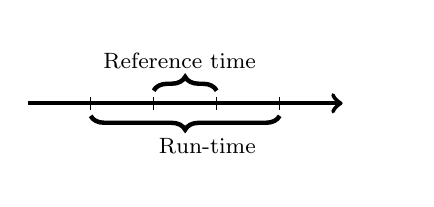
\begin{tikzpicture}[scale=0.8]
            \draw [use as bounding box, draw=none] (0cm,-1.2cm) rectangle (6cm,1.2cm);
            % draw horizontal line   
            \draw[ultra thick, ->] (0,0) -- (5cm,0);
            %\node at (0,2) {The man};
            % draw node
            \draw[ultra thick] (4,0) node[below=3pt,thick] {} node[above=3pt] {};
            \draw[ultra thick] (6,0) node[below=3pt,thick] {} node[above=3pt] {};
            \draw[ultra thick] (8,0) node[below=3pt, thick] {} node[above=3pt] {};
                         \draw[ultra thick] (10,0) node[below=3pt] {} node[above=3pt] {};
            
            \draw [black, ultra thick ,decorate,decoration={brace,amplitude=5pt}] (2,0.2)  -- (3,0.2) 
                   node [black,midway,above=4pt,xshift=-2pt] {\footnotesize Reference time};
            
            
            \draw [ black, ultra thick,decorate,decoration={brace,amplitude=5pt, mirror}] (1,-0.2) -- (4,-0.2)
                   node [black,midway,below=4pt,xshift=8pt] {\footnotesize Run-time};


            % draw vertical lines
            \foreach \x in {1,2,3,4}
            \draw (\x cm,3pt) -- (\x cm,-3pt);
            \end{tikzpicture} & atelic & unbounded \\ \hline
            The man ran. &     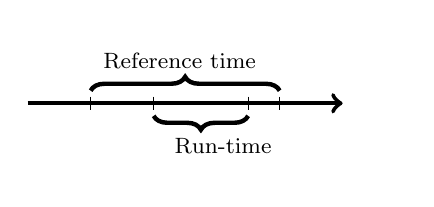
\begin{tikzpicture}[scale=0.8]
                % draw horizontal line   
                \draw [use as bounding box, draw=none] (0cm,-1.2cm) rectangle (6cm,1.2cm);
                \draw[ultra thick, ->] (0,0) -- (5cm,0);
        
                %\draw[node at (0,2) {The man was building a house.}];
                %\node at (0,2) {The man};
        
                % draw node
                \draw[ultra thick] (4,0) node[below=3pt,thick] {} node[above=3pt] {};
                \draw[ultra thick] (6,0) node[below=3pt,thick] {} node[above=3pt] {};
                \draw[ultra thick] (8,0) node[below=3pt, thick] {} node[above=3pt] {};
                             \draw[ultra thick] (10,0) node[below=3pt] {} node[above=3pt] {};
                
                \draw [black, ultra thick ,decorate,decoration={brace,amplitude=5pt}] (1,0.2)  -- (4,0.2) 
                       node [black,midway,above=4pt,xshift=-2pt] {\footnotesize Reference time};
                
                
                \draw [ black, ultra thick,decorate,decoration={brace,amplitude=5pt, mirror}] (2,-0.2) -- (3.5,-0.2)
                       node [black,midway,below=4pt,xshift=8pt] {\footnotesize Run-time};

                            % draw vertical lines
            \foreach \x in {1,2,3.5,4}
            \draw (\x cm,3pt) -- (\x cm,-3pt);
                \end{tikzpicture} & atelic & bounded \\ \hline
            The man was building a house. & 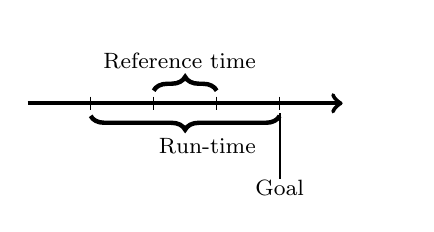
\begin{tikzpicture}[scale=0.8]
                \draw [use as bounding box, draw=none] (0cm,-1.6cm) rectangle (6cm,1.2cm);
                % draw horizontal line   
                \draw[ultra thick, ->] (0,0) -- (5cm,0);
                %\node at (0,2) {The man};
                % draw node
                \draw[ultra thick] (4,0) node[below=3pt,thick] {} node[above=3pt] {};
                \draw[ultra thick] (6,0) node[below=3pt,thick] {} node[above=3pt] {};
                \draw[ultra thick] (8,0) node[below=3pt, thick] {} node[above=3pt] {};
                             \draw[ultra thick] (10,0) node[below=3pt] {} node[above=3pt] {};
                
                \draw [black, ultra thick ,decorate,decoration={brace,amplitude=5pt}] (2,0.2)  -- (3,0.2) 
                       node [black,midway,above=4pt,xshift=-2pt] {\footnotesize Reference time};
                
                
                \draw [ black, ultra thick,decorate,decoration={brace,amplitude=5pt, mirror}] (1,-0.2) -- (4,-0.2)
                       node [black,midway,below=4pt,xshift=8pt] {\footnotesize Run-time};



                            % draw vertical lines
            \foreach \x in {1,2,3,4}
            \draw (\x cm,3pt) -- (\x cm,-3pt);

            \node[align=center] at (4,-1.35) {\footnotesize Goal};
            \draw [thick] (4,-1.2) -- (4,-0.15);
                \end{tikzpicture} & telic & unbounded \\ \hline
            The man built a house. & 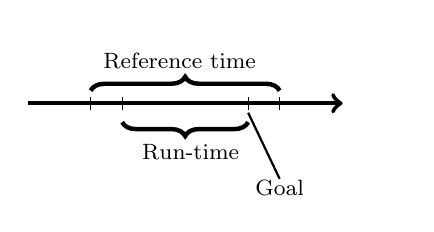
\begin{tikzpicture}[scale=0.8]
                % draw horizontal line   
                \draw [use as bounding box, draw=none] (0cm,-1.6cm) rectangle (6cm,1.2cm);
                \draw[ultra thick, ->] (0,0) -- (5cm,0);
        
                %\draw[node at (0,2) {The man was building a house.}];
                %\node at (0,2) {The man};
        
                % draw node
                \draw[ultra thick] (4,0) node[below=3pt,thick] {} node[above=3pt] {};
                \draw[ultra thick] (6,0) node[below=3pt,thick] {} node[above=3pt] {};
                \draw[ultra thick] (8,0) node[below=3pt, thick] {} node[above=3pt] {};
                             \draw[ultra thick] (10,0) node[below=3pt] {} node[above=3pt] {};
                
                \draw [black, ultra thick ,decorate,decoration={brace,amplitude=5pt}] (1,0.2)  -- (4,0.2) 
                       node [black,midway,above=4pt,xshift=-2pt] {\footnotesize Reference time};
                
                
                \draw [ black, ultra thick,decorate,decoration={brace,amplitude=5pt, mirror}] (1.5,-0.3) -- (3.5,-0.3)
                       node [black,midway,below=4pt,xshift=2pt] {\footnotesize Run-time};

                            % draw vertical lines
            \foreach \x in {1,1.5,3.5,4}
            \draw (\x cm,3pt) -- (\x cm,-3pt);

            \node[align=center] at (4,-1.35) {\footnotesize Goal};
            \draw [thick] (4,-1.2) -- (3.5,-0.15);
                \end{tikzpicture} & telic & bounded \\ \hline
    \end{tabular}
    \caption{Representation of (\ref{para1}),(\ref{para2}),(\ref{para3}) and (\ref{para4}) with regards to the reference time referred to by the utterance and inherent run-time of the event. Concept adapted from \citet{10.1093/oxfordhb/9780199601264.013.25}.}
\end{table}
\label{table:runreftime}

\subsection*{Stativity}
Another parameter of lexical aspect I would like to discuss is stativity, which describes a state of being such as "know", "love" or "be", rather than an action \citep{binnick1991time}. A classic test for stativity in English is non-admittance of the progressive or the imperative \citep{McINTOSH+1975+35+42}.\footnote{Interestingly, however, \citet{Granath_Wherrity_2013} find that, assuming a functional-semantic definition if stativity, the usage of stative verbs with the progressive is much higher in spoken language, than in written language.} Consider the following examples:
\begin{exe}
    \ex[]{She resembles her grandmother.}
    \ex[*]{She is resembling her grandmother.}
\end{exe}
\subsection*{Durativity}
Durativity denotes whether an event takes time (i.e. has duration) or happens in an instant, and this can be checked in English by the compatibility of durative adverbs such as \emph{for an hour} \citep{102998}. For example:
\begin{exe}
    \ex[]{Andrea was painting a picture for an hour.}
    \ex[*]{Andrea was reaching the summit for an hour.}
\end{exe}
\subsubsection{Some attempts at event classification}
\subsection*{\citet{vendler57}}
It was the seminal work \emph{Verbs and Times} \citep{vendler57} of philosopher Zeno Vender which initiated the discussion on inner aspect in the linguistic tradition.\footnote{A similar classification was also developed independently by Anthony Kenny in \emph{Action, Emotion and Will} \citep{Kenny1963-KENAEA}, however combining Achievement and Accomplishment into one single class \citep{19c36731-bdec-362e-9f45-1aaba76109d7}. Hence it is sometimes referred to as the Vendler-Kenny scheme of verb-types.} Vendler begins his discussion with the following premise:

\begin{displayquote}
    Indeed, as I intend to show, if we focus our attention primarily upon the time schemata presupposed by various verbs, we are able to throw light on some of the obscurities which still remain in these matters. [...] There are a few such schemata of very wide application. Once they have been discovered in some typical examples, they may be used as models of comparison in exploring and clarifying the behavious of any verb whatever.\footnote{\citet{vendler57}}
\end{displayquote}
That is to say, the "time schema" of any verb can be described through comparison with a set of prototypical classes (see \ref{table:vendlerverbs}), which can be easily identified. In order to arrive at these prototypical "schemata" he uses an analytical method consisting of classifying verbs according to their behaviour regarding certain elements of English grammar, as was also used to outline the aspectual parameters above.\footnote{The issue of Anglocentrism is one which has plagued many a linguistic theory throughout the years, with work from Chomsky's generative grammar \citep{LEVISEN2019101173} to Abstract Meaning Representation \citep{damonte2018crosslingual} being criticised for their too heavy focus on English.} For example, the first distinction he makes is between English verbs that permit the progressive and those that don't. This signals the first class of events known as 'states'. The article then goes on to outline the other three Vendlerian classes \emph{activity, accomplishment} and \emph{achievement}, and their character is summarised thus: 

\begin{itemize}
    \item \textbf{State} - non-dynamic, static and durative situation
    \item \textbf{Activity} - open-ended, dynamic and durative processes without an end-point
    \item \textbf{Accomplishment} - dynamic and durative processes with a natural end-point
    \item \textbf{Achievement} - instantaneous or near-instantaneous events (such as semelfactives)
\end{itemize}

Or to use the parameters of lexical aspect introduced above:
\begin{table}
    \centering
    \begin{tabular}{|c||c|c|c|}
        \hline
                                & Static & Durative & Telic \\ \hline
        \textbf{State}          & +      & +        & - \\ \hline
        \textbf{Activity}       & -      & +        & - \\ \hline
        \textbf{Accomplishment} & -      & +        & + \\ \hline
        \textbf{Achievement}    & -      & -        & + \\ \hline
    \end{tabular}
    \caption{Classification of Vendlerian event types by binary aspectual parameters \citep{Smith1991ThePO}.}
\end{table}

Vendler states in his introduction that verbs "presuppose" certain time schemata and hence assigns a category to each verb (as in \ref{table:vendlerverbs}). However it must also be stated that the true profile of a verb phrase such as those listed in \ref{table:vendlerverbs} depends heavily on the context. Hence a typical semelfactive such as "sneeze" could also be used reinterpreted as a process when combined with a progressive auxiliary as in "Harry was sneezing" \citep{moens-steedman-1988-temporal}. Thus the verbs (or verb phrases) mentioned by Vendler as belonging to a certain category are ones that typically lend themselves to one class or another.

\begin{table}
    \centering
    \begin{tabular}{|c|c|c|c|}
        
        \textbf{State} & \textbf{Activity} & \textbf{Accomplishment} & \textbf{Achievement} \\
        know & running & paint a picture & reach the summit \\
        understand & pushing & build a house & spot the plane \\
        love & smoking & deliver a sermon & recognise
    \end{tabular}
    \caption{Some of the example verb phrases given in \citet{vendler57} for the classification of events.}
\end{table}
\label{table:vendlerverbs}

\subsection*{\citet{moens-steedman-1988-temporal}}

\subsection{Grammatical aspect}
Grammatical (or \emph{viewpoint}) aspect provides a lens through which a particular event is viewed and it "is typically expressed by overt grammatical morphemes (hence the label grammatical aspect)" \citep{Chapter1IntroductionCrossLinguisticPerspectivesontheSemanticsofGrammaticalAspect}. \citet{comrie1976aspect} provides a hierarchical classification of aspectual oppositions shown in \ref{fig:comrieaspecttree}, and in the following section I will briefly describe some of the main oppositions described in this classification: the perfective vs. imperfective opposition and habituality, 

\begin{figure}
    \centering
    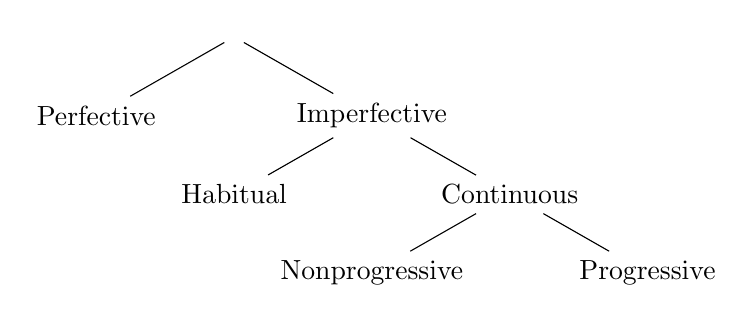
\begin{tikzpicture}
        \node {}[sibling distance = 3.5cm, level distance = 1cm]
        child [black] {node {Perfective} 
            edge from parent [black] node [left] {}}
        child {node {Imperfective} 
            child [black] {node {Habitual}
                edge from parent [black] node [left] {}}
            child [black] {node {Continuous}
                child [black] {node {Nonprogressive}
                    edge from parent [black] node [left] {}}
                child [black] {node {Progressive}
                    edge from parent [black] node [right] {}}
                edge from parent [black] node [right] {}} 
            edge from parent [black] node [right] {}};
    \end{tikzpicture}
    \caption{Comrie's classification of aspectual oppositions. Reproduced from \citet{comrie1976aspect}.}
    \label{fig:comrieaspecttree}
\end{figure}

\subsection*{Perfectivity}
\label{sec:perfectivity}
The main aspectual distinction made by Slavic languages and, as can bee seen in figure \ref{fig:comrieaspecttree}, one of the main distinctions made in theoretical aspectology generally as that between perfective and imperfective. As noted by \citet{Dahl1985TenseAA}, the theoretical distinction between perfectivity and imperfectivity is different to their concrete realisation in the Slavic language group. To avoid confusion, I will therefore henceforth use the terms to 'perfective' and 'imperfective' to refer to the theoretical binary opposition, and only refer to the Slavic (im-)perfectivity explicitly.

Returning to the definition of grammatical aspect as \emph{situation-internal} but \emph{event-external} (REFERENCE), perfectivity can be seen as a focus on the event as a whole indivisible entity (i.e. its result), and imperfectivity implies a focus on its internal temporal constituency \citep{comrie1976aspect, wals-65}. In practice this often means that perfective verbs refer to "completed" events (EXAMPLE), and imperfective verbs to incomplete or long-lasting events (EXAMPLE), however note that this is not always the case.

\subsection*{Habituality}

\section{Aspect in Slavic languages}
The Slavic language group has a special place on the study of aspectology due to its overt encoding of aspectual phenomena, otherwise rather uncommon \citep{slavstyleaspect}.\footnote{\citet{slavstyleaspect} also notes that Georgian and Ossetian exhibit some similar properties with preverbs (mostly of spatial origin) used to denote aspectual meaning.} Verbs in Slavic languages, with few exceptions (CHECK IF THIS IS TRUE), are either perfective or imperfective, meaning the speaker must explicitly state the aspect of the verb event referenced. 

\begin{exe}
    \ex Ja proCCitaju Etu knigu.
\end{exe}

(HOW DO I DO THE GLOSSING HERE)

As mentioned, the opposition between these two lexical categories differs slightly from the "purer" theoretical distinction discussed in \ref{sec:perfectivity}. A classic example where the usage does not correspond to the WHAT is the pair \ref{oknoperf} and \ref{oknoimp}, where the former is a prototypical usage of the perfective to denote a whole completed event, the latter imperfective form denotes that the event has since been undone (CHECK THIS) \citep{franks2005slavic}.

\begin{exe}
    \ex Kto otkryl okno?
    \label{oknoperf}
    \ex Kto otkryval okno?
    \label{oknoimp}
\end{exe}

It is also interesting to note that modern Slavic aspect, now usually seen as a \emph{grammatical} feature, developed from spatial prefixes ??? The most common perfectivising prefix \emph{po-} used to refer to WHAT, however has slowly developed into a temporal marker and finally into a grammatical aspect marker.

The diachronic (GRADUAL?) grammaticalisation of lexemes exhibited by Slavic languages is further evidence in favour of a less clear distinction between grammatical and lexical aspect.
WE CAN SEE THE DIACHRONICAL DEVELOPMENT FROM LEXICAL ASPECT TO GRAMMATICAL ASPECT

It is due to this covert aspect marking that I decided to include Slavic languages in this study, and 


\section{Aspectual ambiguity}
While some verb phrases can only express one certain aspect, such as \emph{to tend to}, which implies a habitual event, in many situations they can be ambiguous:
\begin{exe}
    \ex Your soul was made to be \textbf{filled} with God Himself. \emph{(Brown corpus, cited by \citet{Friedrich2014AutomaticPO})}
\end{exe}
In this example the verb 'filled' can be read as both a stative and a dynamic event.\footnote{Indeed, while not specified in English, this is explicitly encoded in other languages such as German where the former interpretation would use the word \emph{sein} (to be) and the latter \emph{werden} (to become).} Nevertheless, in many cases the reader tends to prefer a particular interpretation, such as in \ref{walktoschoolsent}, where the sentence is most likely to be a habitual, a common use of the English simple present, and yet could also be interpreted as a narrative present (RIGHT NAME?) as in \ref{walktoschoolsent2}.

\begin{exe}
    \ex He walks to school.
    \label{walktoschoolsent}
    \ex He walks off to school.
    \label{walktoschoolsent2}
\end{exe}


This poses a practical problem for annotators when asked to provide a single class for a sentence (or sometimes even just for a verb phrase as in \citet{siegel-mckeown-2000-learning}), but also an interesting theoretical question for linguists. For simplicity, most studies have assumed that ASPECT IS EINDEUTIG!!. There have been no studies on aspect ambiguity as of yet \citep{friedrich-etal-2023-kind}, despite this being a not too uncommon occurrence in language (see \ref{sec:dataset_creation}). Some, such as \citet{umr} (see \ref{aspect_in_umr}), have got around this problem by classifying aspect in a lattice structure, allowing for more coarse grained categories when necessary. While perhaps doable in practice, this is in unsatisfactory solution to describe to several semantically distinct interpretations of a particular utterance.

\subtitle{Contexts frequently triggering aspectual ambiguity in English}
WHAT ARE THE CIRCUMSTANCES IN WHICH AMBIGUITY ARISES IN ENGLISH?

taking out the habitual of course

semelfactives (single / iterative)
passive (stativity / dynamicity) -> how is this in Russian?
past simple (stativity / dynamicity)
Verbs of motion with ambiguous prepositions (telic / atelic)

see - Coercion and underspecification integrated: The state-event ambiguity of aspectual verbs (past simple); Automatic prediction of aspectual class of verbs in context (passive stative / dynamic)

While not directly encoding dynamicity, telicity or iterativity, the choice of perfective / imperfective in Slavic languages is strongly influenced by boundedness and whether an event is a single situation or repeated \citep{wiemer2017}. While the latter equates to iterativity, boundedness is also highly correlated with telicity and stativity (?), and hence the (obligatory) choice of PERF/IMPF forces one of the two possible interpretations in each case. \citet{errors_in_russian_aspect_apresyan} also finds that L2 Russian speakers are more likely to choose the incorrect aspect if their L1 does not differentiate between these two interpretations in a particular case, corroborating intuition.

\subsection{Coercion or underspecification?}
\ref{walktoschoolsent} and \ref{walktoschoolsent2} are an example of how, unless further specified, a verb phrase in a sentence can tend towards a particular aspectual interpretation, however further specification leads to a different interpretation. In cases where a verb can have several aspect readings depending on the context, a question that currently remains unclear is whether verbs have an inherent aspect class, which is \emph{overwritten} by the features of the context is occurs in (temporal adverbs, other verb phrases forcing a particular class such as \emph{to tend to} etc.), or whether they are simply underspecified in the mental lexicon, and the class is \emph{determined} by these circumstantial features \citep{https://doi.org/10.11588/huplc.2017.0.37820}. The former view, as put forward by \citet{moens-steedman-1988-temporal} and known as \emph{coercion}, is used as an assumption in many previous works (cf. \citet{Swart+2019+321+349}) with little evidence of its validity \citep{https://doi.org/10.11588/huplc.2017.0.37820}. It is therefore an open question how both humans and language models deal with this aspectual conflict. The following study will aim to shed some light on the behaviour of the latter in such situations, and perhaps provide some insight into the possible mechanisms of the former.

\section{Formal models of aspect (or put this in related work?)}
Finally, I would like to outline some of the formal logical approaches that have been made in this area